\documentclass{beamer}
%\usepackage{xcolor}
%\usepackage{beamerthemesplit}
\usepackage{amscd}
\usepackage{graphicx}
%\usepackage{pgf}


%\usetheme[headhight=10, footheight=10]{}
%gets rid of bottom navigation bars
\setbeamertemplate{footline}{}

%gets rid of navigation symbols
\setbeamertemplate{navigation symbols}{}

\definecolor{olive}{rgb}{0.3, 0.4, .1}
\definecolor{fore}{RGB}{249,242,215}
\definecolor{back}{RGB}{51,51,51}
\definecolor{title}{RGB}{255,0,90}
\definecolor{dgreen}{rgb}{0.,0.6,0.}
\definecolor{gold}{rgb}{1.,0.84,0.}
\definecolor{JungleGreen}{cmyk}{0.99,0,0.52,0}
\definecolor{BlueGreen}{cmyk}{0.85,0,0.33,0}
\definecolor{RawSienna}{cmyk}{0,0.72,1,0.45}
\definecolor{Magenta}{cmyk}{0,1,0,0}

\def\Z{\mathbb{Z}}
\def\R{\mathbb{R}}
\def\Q{\mathbb{Q}}
\def\H{\mathbb{H}}
\def\HH{\mathcal{H}}
\def\E{\mathbb{E}}
\def\N{\mathbb{N}}
\def\P{\mathbb{P}}
\def\PC{{\mathbb{P}C}}
\def\CP{\mathbb{CP}}
\def\C{\mathbb{C}}
\def\L{\mathcal{L}}
\def\PSL{\textnormal{PSL}}
\def\GL{\textnormal{GL}}
\def\Aut{\textnormal{Aut}}
\def\1{\boldsymbol{1}}
\newtheorem{proposition}{Proposition}
\newtheorem{question}{Question}
\newtheorem{answer}{Answer}
\newtheorem{conjecture}{Conjecture}

\title{Kleinian groups and 3-Manifolds}
\author{Danny Calegari}
\date{February 28 2014}

\begin{document}

\frame{\titlepage}
\frame
{
\frametitle{1. Kleinian groups}

A \textcolor{blue}{Kleinian group} is a \textcolor{red}{finitely generated} and 
\textcolor{red}{discrete} group of \textcolor{red}{conformal} symmetries of the 
\textcolor{dgreen}{sphere}, where

\begin{enumerate}
\item{``the \textcolor{dgreen}{sphere}'' means the round unit sphere in Euclidean 3-space; and}
\item{``\textcolor{red}{conformal}'' means smooth maps which preserve angles.}
\end{enumerate}

The collection of all conformal symmetries of the sphere is a \textcolor{blue}{Lie group}; ``\textcolor{red}{discrete}''
means discrete as a subset of this group.
}
\frame
{
\begin{columns}[c]
\column{1in}
A \textcolor{red}{finite group} of
rotations is a Kleinian group.
\column{3in}
\begin{center}
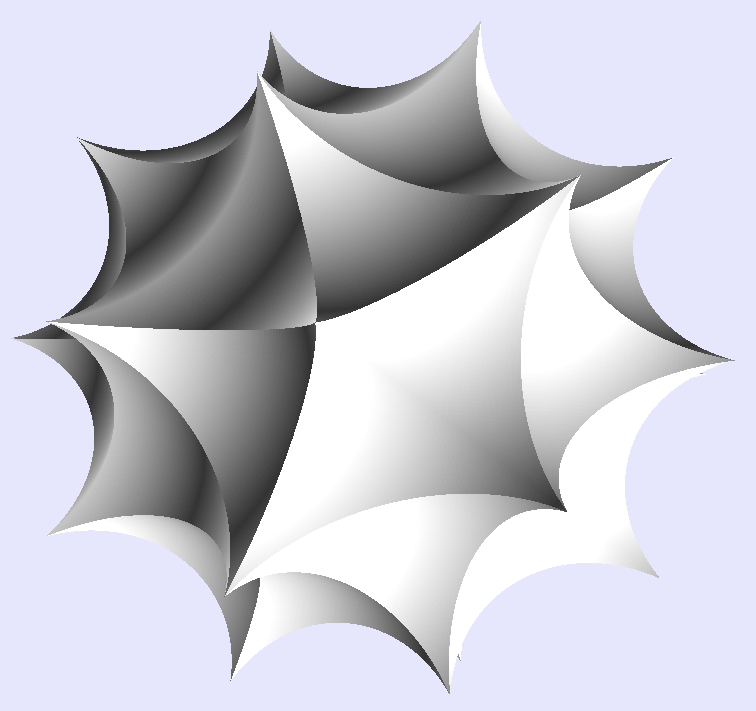
\includegraphics[width=3in]{icosahedron.png}
\end{center}
\end{columns}
}
\frame
{
\begin{columns}[c]
\column{1.1in}
The symmetries of a 
\textcolor{red}{Euclidean tessellation}
is a Kleinian group
by stereographic
projection.
\column{3in}
\begin{center}
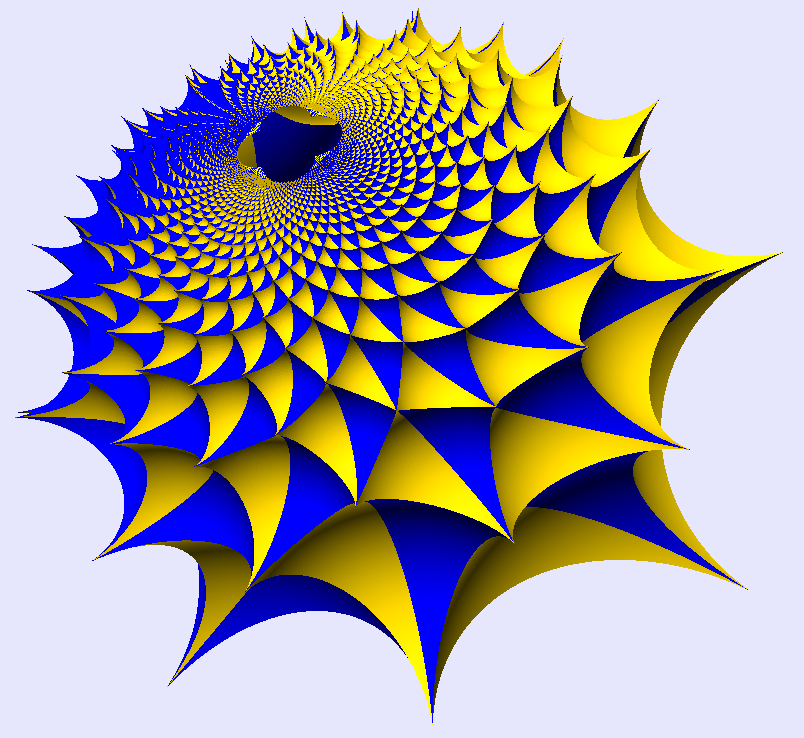
\includegraphics[width=3in]{parabolic.png}
\end{center}
\end{columns}
}
\frame
{
\begin{columns}[c]
\column{1.1in}
A Kleinian group 
preserving a round circle
on the sphere is a
\textcolor{blue}{Fuchsian group}.
\column{3in}
\begin{center}
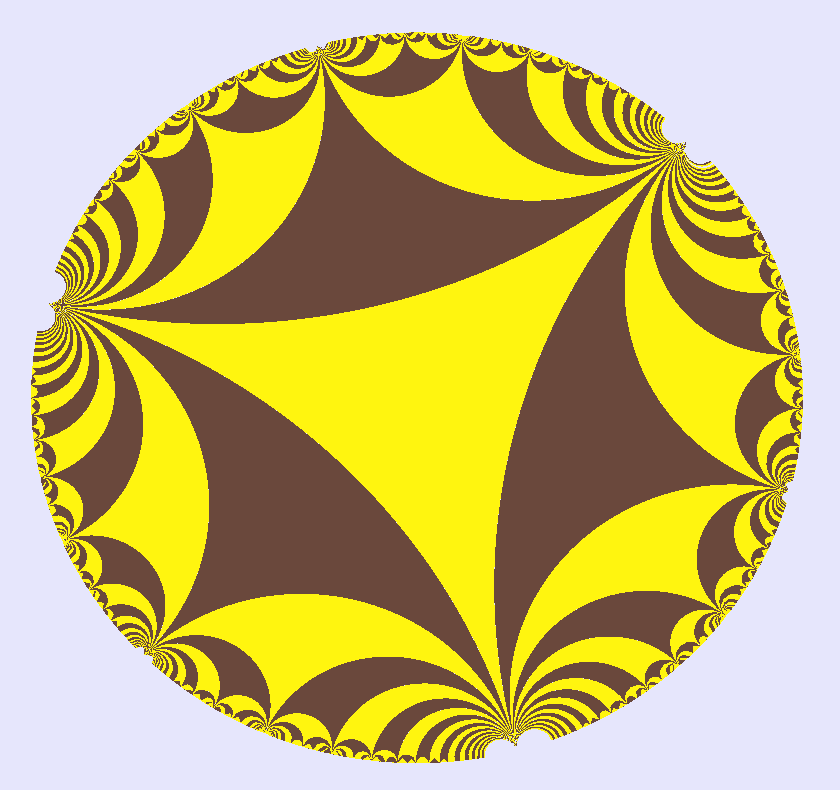
\includegraphics[width=3in]{fuchsian.png}
\end{center}
\end{columns}
}
\frame
{
If we identify the unit sphere with the \textcolor{dgreen}{Riemann sphere} 
$$S^2 = \CP^1:=\C\cup \infty$$
then (orientation-preserving) conformal symmetries are \textcolor{red}{fractional linear
transformations}
$$z \to \frac {az+b} {cz+d}$$
and the group of all such transformations is $\PSL(2,\C)$.
}
\frame
{
\frametitle{2. Differential Equations}

Kleinian groups arise in nature as monodromy groups of \textcolor{dgreen}{differential equations}.
\vskip 5pt
Euler introduced the \textcolor{blue}{hypergeometric equation}
$$z(1-z)\frac {d^2w}{dz^2} + [c - (a+b+1)z]\frac {dw}{dz} - abw = 0$$
where $w$ is a function of the variable $z$, and $a$, $b$, $c$ are real constants.
\vskip 10pt
For Euler, $w$ and $z$ were real; but for us they can be complex numbers.
}
\frame
{The space of solutions to the hypergeometric equation
is a complex vector space $V$ of dimension 2. 
\vskip 10pt
There are \textcolor{dgreen}{regular singular points}
at $0$, $1$ and $\infty$, and solutions may be \textcolor{red}{analytically continued} 
around these points.
\vskip 10pt
If $f$ and $g$ are a basis for $V$, the map $$D:z \to f(z)/g(z)$$ is well-defined
in the \textcolor{dgreen}{upper half plane}
$$\HH:=\lbrace z \in \C \text{ with positive imaginary part} \rbrace$$
}
\frame
{
Schwarz showed that the image $D(\HH)$ is a \textcolor{dgreen}{curvilinear triangle} $T$ in $\C$
whose sides are segments of \textcolor{red}{round circles} or \textcolor{red}{straight lines}
and whose angles are $|1-c|\pi$, $|c-a-b|\pi$ and $|a-b|\pi$.
\vskip 10pt
If we \textcolor{red}{analytically continue} $D$ across a segment of 
$\R - \lbrace 0,1,\infty\rbrace$, it maps
the lower half plane $\overline{\HH}$ onto a triangle obtained from $T$ by \textcolor{dgreen}{inversion}
in the corresponding circular side. 
\vskip 10pt
Continuing $D$ around loops, we get a
representation 
$$D_*:\pi_1(\CP^1 - \lbrace 0,1,\infty\rbrace) \to \PSL(2,\C)$$ 
}
\frame
{
If the angles of the curvilinear triangle are of the form $\pi/n$ for integers $n$, 
the image is discrete, and hence a Kleinian group
called a \textcolor{blue}{triangle group}.
\begin{center}
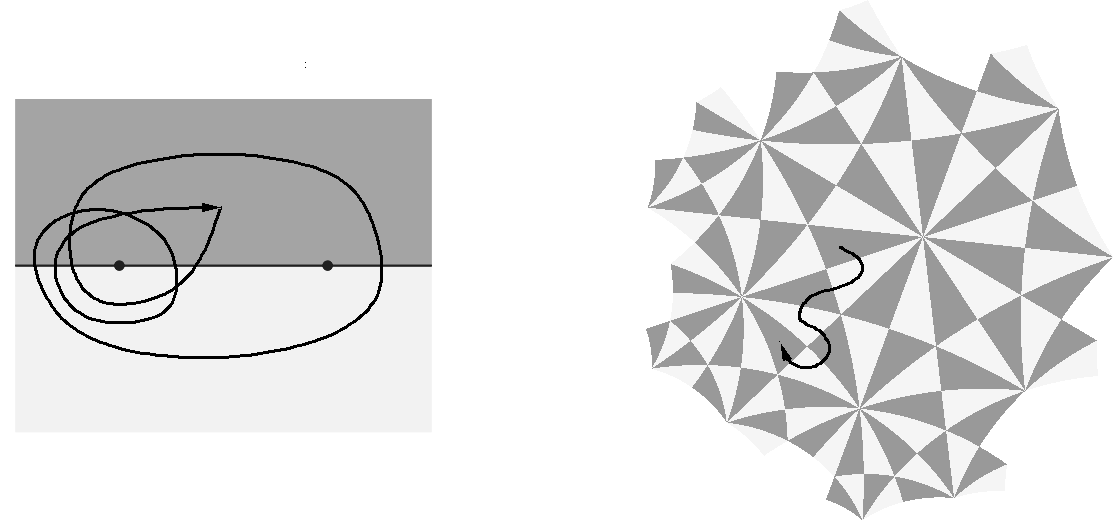
\includegraphics[width=4in]{triangle_group.png}
\end{center}
}
\frame
{
\frametitle{3. Hyperbolic geometry}
Poincar\'e realized that $\PSL(2,\C)$ is also the group
of (orientation-preserving) \textcolor{red}{isometries} of hyperbolic 3-space $\H^3$.
\vskip 10pt
In Poincar\'e's model, $\H^3$ is the interior of the unit ball.
The hyperbolic metric is obtained by rescaling the Euclidean metric
by a factor of $2/(1-r^2)$ where $r$ is the distance to $0$.
\vskip 10pt
Straight lines in the Poincar\'e metric are arcs of Euclidean
straight lines or circles perpendicular to the boundary sphere.
}
\frame
{
\begin{columns}[c]
\column{1.1in}
In the Poincar\'e
metric, objects near the
boundary sphere look
smaller.
\column{3in}
\begin{center}
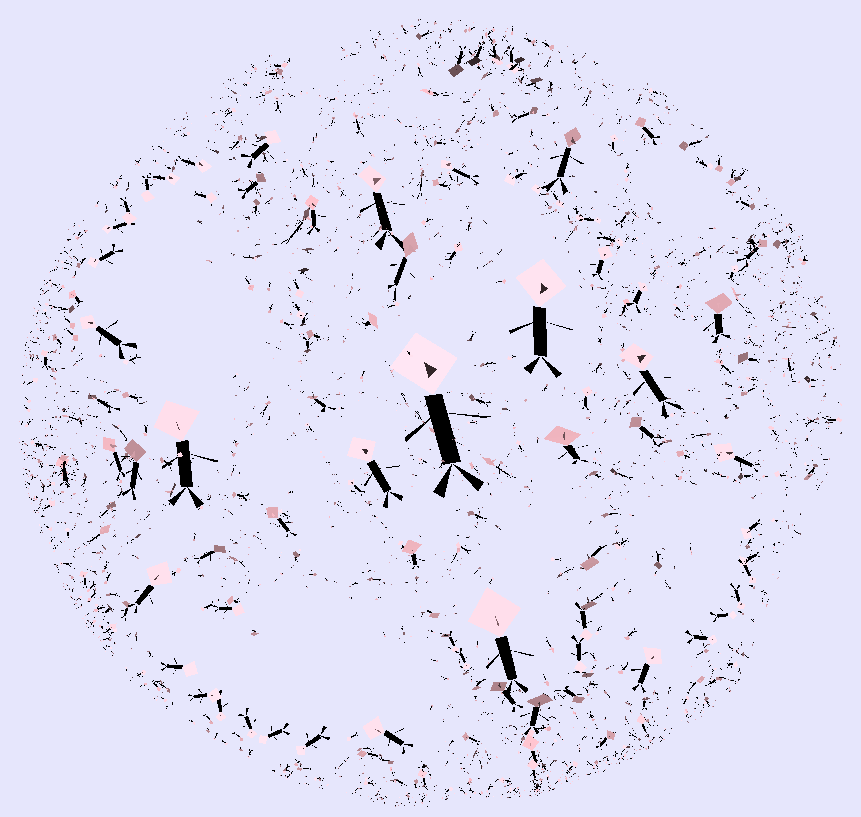
\includegraphics[width=3in]{Poincare.png}
\end{center}
\end{columns}
}
\frame
{
If $\Gamma$ is a torsion-free Kleinian group, then
$\Gamma$ acts \textcolor{red}{freely} and \textcolor{red}{properly discontinuously}
on $\H^3$ by isometries.
\vskip 10pt
Thus the quotient $M:=\H^3/\Gamma$ is a \textcolor{blue}{hyperbolic manifold}
with universal cover $\H^3$, and fundamental group $\pi_1(M)\cong \Gamma$.
}
\frame
{
\frametitle{4. Limit sets}
If $\Gamma$ is a Kleinian group, the sphere $S^2$ decomposes into 
\begin{enumerate}
\item{the \textcolor{blue}{Limit set} 
$\Lambda$ where $\Gamma$ acts \textcolor{red}{ergodically}, and}
\item{the \textcolor{blue}{Domain of discontinuity}
$\Omega$ where $\Gamma$ acts \textcolor{red}{properly discontinuously}.}
\end{enumerate}
$\Lambda$ is closed, and $\Omega$ is open. For most Kleinian groups, $\Lambda$ is the closure
of the set of fixed points of $\Gamma$.
\vskip 10pt
The quotient $\Omega/\Gamma$ is a Riemann surface. Ahlfors showed it is of
\textcolor{dgreen}{finite type}; i.e.\/ it is homeomorphic to a compact surface
minus finitely many points.
}
\frame
{
\begin{block}{References}
\begin{itemize}
\item{D. Mumford, C. Series and D. Wright, {\em Indra's Pearls: The Vision of Felix Klein}.}
\item{W. Thurston, {\em Three dimensional manifolds, Kleinian groups and hyperbolic geometry},
Bull. AMS, 1982}
\end{itemize}
\end{block}
}

\end{document}

